% Compiler: LaTeX => PDF

\documentclass{beamer}

\usepackage[ngerman]{babel}
\usepackage[utf8]{inputenc}

%\usepackage{multimedia}
\usepackage{graphicx}
\usepackage[nolist]{acronym}

\usepackage{stackengine}
\usepackage{array}

\usepackage{enumitem}

\setitemize{label=\usebeamerfont*{itemize item}%
  \usebeamercolor[fg]{itemize item}
  \usebeamertemplate{itemize item}}

\title{Streifenprojektion}
%\subtitle{X $\in \{$ Motion, Shading, Texture $\}$}
%\subtitle{Schwerpunkte: Shape from Motion, \\ Shape from Shading, Shape from Texture}
\author{Dennis Wagner, \\ Johannes Spangenberg, \\ Leroy Kramer}
%\date{\today}
\date{12.02.2014}

% add page number
\setbeamertemplate{footline}[frame number]

\begin{document}


\frame{\titlepage} 


\begin{frame}
	\frametitle{Gliederung}
	\tableofcontents
\end{frame} 


\section{0 \hspace{5px} Unsere Aufgabe} 
\begin{frame}
	\frametitle{Streifenprojektion}
	\framesubtitle{Unsere Aufgabe}

	[Foto eines Setups]

\end{frame}


\subsection{0.1 \hspace{5px} Motivation} 
\begin{frame}
	\frametitle{Streifenprojektion}
	\framesubtitle{Motivation}

	\begin{itemize}
		\item günstige Methode um Vermessungen durchzuführen
	\end{itemize}

\end{frame}

% ---------------------------------------------------------------------------- %

\section{1 \hspace{5px} Umsetzung} 
%\subsection{1.1 \hspace{5px} Hardware}
\begin{frame}
	\frametitle{Streifenprojektion}
	\framesubtitle{Umsetzung}

	\includegraphics[width=0.9\linewidth]{includes/hardware.jpg}

\end{frame}


%\subsection{1.1 \hspace{5px} Software}
\begin{frame}
	\frametitle{Streifenprojektion}
	\framesubtitle{Umsetzung}

	
	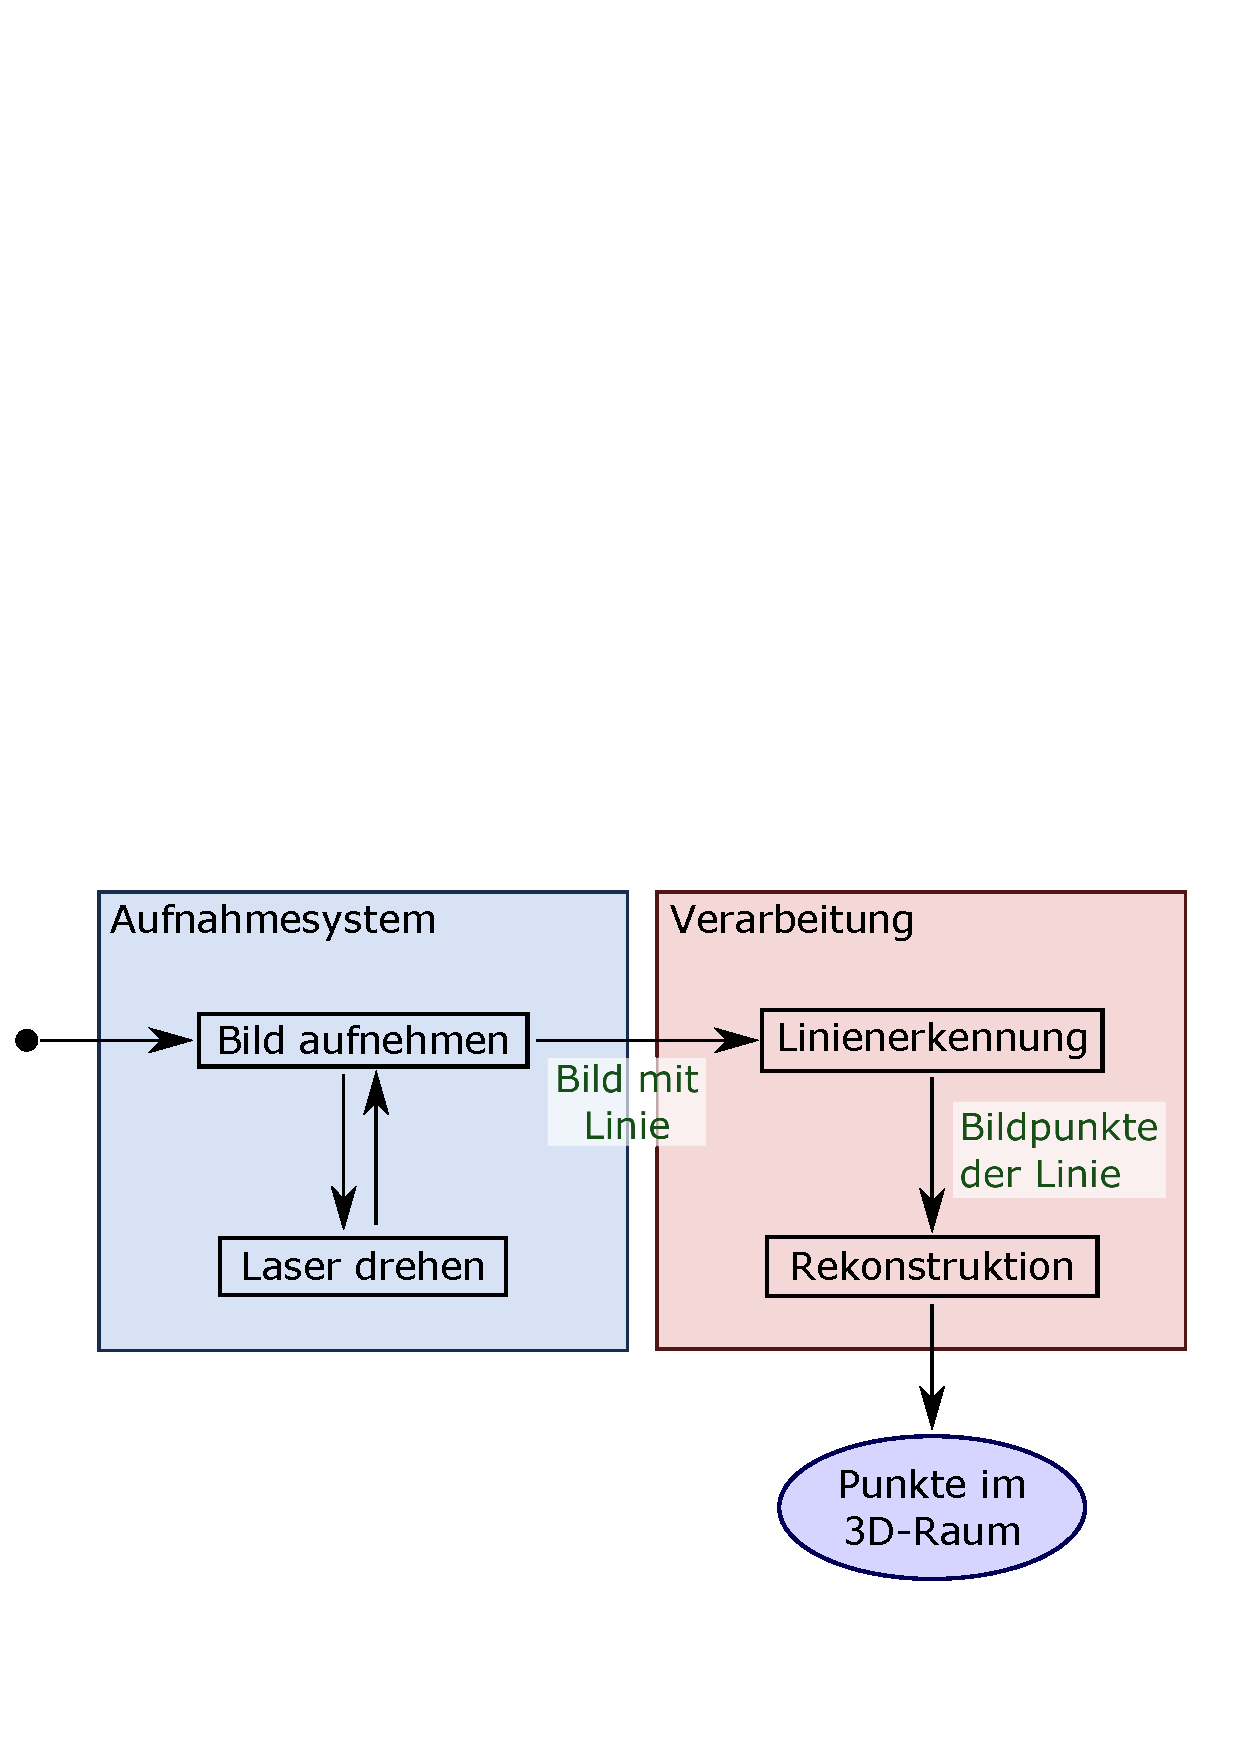
\includegraphics[width=\linewidth]{includes/blockbild.png}

\end{frame}


\section{2 \hspace{5px} Probleme}
\begin{frame}
	\frametitle{Streifenprojektion}
	\framesubtitle{Probleme}

	\begin{itemize}
		\item Viel Zeit bei Planung verloren
		\item Uneinigkeit bei der Wahl der Verfahren
	\end{itemize}

\end{frame}

\subsection{2.1 \hspace{5px} bei der Hardware}
\begin{frame}
	\frametitle{Streifenprojektion}
	\framesubtitle{Probleme bei der Hardware}

	\begin{itemize}
		\item Aufbau der Hardware
		\begin{itemize}
			\item Montage von Laser auf Servo
			\item Montage der Kamera
		\end{itemize}
		\item Ursache für Ungenauigkeiten
		\begin{itemize}
			\item kleine Fehler bei der Montage können u.U. zu großen Fehlern führen
			\item schwer die Winkel und Entfernungen von/zwischen Kamera, Servo und Laser genau zu messen 
		\end{itemize}
	\end{itemize}

\end{frame}

\begin{frame}
	\frametitle{Streifenprojektion}
	\framesubtitle{Probleme}

	\includegraphics[width=\linewidth]{includes/krumm.png}

\end{frame}

\subsection{2.1 \hspace{5px} bei der Linienerkennung}
\begin{frame}
	\frametitle{Streifenprojektion}
	\framesubtitle{Probleme bei der Linienerkennung}

	\begin{itemize}
		\item Lücken
		\item Hintergrundfarbe
	\end{itemize}

\end{frame}

\section{Ergebnisse}

\subsection{wiederholte Vesuche}


\subsection{verschiedene Farben}
\begin{frame}
	\frametitle{Streifenprojektion}
	\framesubtitle{Ergebnisse}

	Reale Höhe: 56mm
	\begin{tabular}{c|c|c|c}
		Farbe & Hoehe (mm) & Abweichung (mm) & Abweichung (\%) \\
		Blau & 55.0 & -1 & -1.8\\
		Grün & 57.0 & 1 & 1.8\\
		Orange & 54.5 & -1.5 & -2.7\\
		Rot & 55.4 & -0.6 & -1.1\\
		Weise & 56.6 & 0.6 & 1.1\\
		Gelb & 54.8 & -1.2 & -2.1	
	\end{tabular}

\end{frame}

\begin{frame}
	\frametitle{Streifenprojektion}
	\framesubtitle{Ergebnisse}

	Reale Entfernung: 300mm 
	\begin{tabular}{c|c|c|c|c|c}
		Farbe & Min & Max & Avg & Abweichung (mm) & Abweichung (\%)\\
		Blau & 314.9 & 318.8\\
		Grün & 314.9 & 318.9\\
		Orange & 307.2 & 318.9\\
		Rot & 305.3 & 318.9\\
		Weiß & 298.1 & 316.8\\
		Gelb & 284.7 & 320.9
	\end{tabular}

\end{frame}

\subsection{verschiedene Entfernungen}
\begin{frame}
	\frametitle{Streifenprojektion}
	\framesubtitle{Ergebnisse}

	Reale Höhe: 56mm
	\begin{tabular}{c|c|c|c}
		Entfernung & Hoehe & Abweichung (mm) & Abweichung (\%) \\
		150 & 57.1.0 & 1.1 & 2.0\\
		200 & 57.1 & 1.1 & 2.0\\
		250 & 57.4 & 1.4 & 2.5\\
		300 & 57.2 & 1.2 & 2.1\\
		350 & 56.4 & 0.4 & 0.7
	\end{tabular}

\end{frame}

\begin{frame}
	\frametitle{Streifenprojektion}
	\framesubtitle{Ergebnisse}

	\begin{tabular}{c|c|c|c|c|c}
		Entfernung & Min & Max & Avg & Abweichung (mm) & Abweichung (\%)\\
		150 & 161.2 & 163.3\\
		200 & 211.0 & 215.5\\
		250 & 262.5 & 268.1\\
		300 & 316.8 & 320.9\\
		350 & 335.8 & 373.0
	\end{tabular}

\end{frame}


\section{3 \hspace{5px} Live-Demo} 
\begin{frame}
	\frametitle{Streifenprojektion}
	\framesubtitle{Live-Demo}

\end{frame}


\section{4 \hspace{5px} Quellen} 
\begin{frame}
	\frametitle{Streifenprojektion}
	\framesubtitle{Quellen}
	
\end{frame}


\end{document}
